\cotefile{69}
\scanpage{3}

% head
\mspage{1}
\uline{Th.} Soit $S$ un graphe tel que

% ll. 2–4
\[
\begin{aligned}
\text{a)}\quad &\operatorname{card} S=27\\
\text{b)}\quad &\forall s\in S,\quad \operatorname{card} E(s)=10\qquad
 (E(s)=\{t\in S\mid t\text{ lié à }s\}\\
\text{c)}\quad &\forall s,t\in S,\quad s,t\text{ liés},\quad
 \exists!u\in S,\quad u\text{ lié à }s\text{ et }t.
\end{aligned}
\]

% l. 5
Alors (et alors seulement) $S$ est un graphe cubique.

% ll. 6–7
\uline{Dém} \unsure{Soit|Soient} $u\in S$, \deleted{$v\in E(s)$} ($\operatorname{card}S\geq27$ !) $v\in E(u)$ i.e. $v$ lié à $u$ ($\operatorname{card} E(u)=10$), $w\in S$ tel que $w$ lié à $u$ et $v$ (axiome c).

% l. 8
On dit que $T=\{u,v,w\}$ est un ``triangle''.

% ll. 9–10
\uline{Lemme 1} Tout $s\in S-\inserted{\unsure{(S^*=\{u,v,w\})|(\{u,v,w\})|\{u,v,w\}=S^*}}$ est lié à un et un seul des él. $u,v,w$ [ i.e. $S^*=S-\{u,v,w\}$ est \uline{réunion} \uline{disj.} de $E(u)^*=S^*\cap E(u),E(v)^*,E(w)^*$ (ch. un de cardinal 8)

% ll. 11–13
Comme $\operatorname{card} E(u)=10$, \deleted{\unsure{si on|tiens}} on a $\operatorname{card}\overbrace{E(u)\cap S^*}^{E(u)^*}=8$ car $E(u)\cap S^*=E(u)-\{v,w\}$, de même \deleted{card} $\overbrace{E(v)\cap S^*}^{\unsure{E(u)^*|E(v)^*}},\ \overbrace{E(w)\cap S^*}^{E(w)^*}$ sont de cardinal 8. Or par c), $E(u)\cap E(v)=\{w\}$ donc

% ll. 14–18
$E(u)^*\cap E(v)^*=\varnothing$ et de $=$ pour les autres 2 couples, donc $E(u)^*,E(v)^*,E(w)^*$ disjoints, donc la \deleted{\unsure{somme}}\inserted{réunion} est de cardinal \deleted{\unsure{24}} $3\times8=24$. Comme $S^*$ est de cardinal $27-3=24$ par a), on trouve que $S^*$ est réunion (disjointe) des $E(u)^*,E(v)^*,E(w)^*$, cqfd.

% ll. 19–20
\uline{Lemme} 2 $\forall x\in \deleted{\unsure{E(u)^*}}S^*$, $\exists!u'\in E(u)^*$ lié à $u$. (De $=$ pour $v,w$). / En effet, \deleted{\unsure{l'unicité est bien|l'unicité}}\inserted{\unsure{c'est une|n'est qu'une|des liés}} reformulation de c)

% ll. 21–23
\uline{Corollaire} $\exists!\sigma=\sigma_T:S\longrightarrow S$ tel que $\sigma_{\unsure{t|T}}$ laisse $u,v,w$ et que $\forall x\in S^*=S-\{u,v,w\}$, $\sigma_T(x)$ soit lié à $x$ et $x$ et $\sigma_{\unsure{t|T}}(x)$ liés au $=$ sommet $u,v,w$ de $T$.

% lower left, beside corollary
\figure{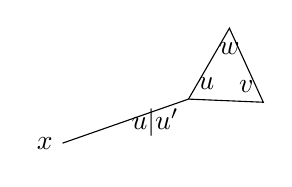
\begin{tikzpicture}[x=1cm,y=1cm]
\draw (0,0) -- (1.60,.56) -- (2.12,1.46) -- (2.55,.52) -- (1.60,.56);
\node[left] at (0,0) {$x$};
\node[below left] at (1.60,.56) {$\unsure{u|u'}$}; \node[above right] at (1.60,.56) {$u$};
\node[below] at (2.12,1.40) {$w$}; \node[above left] at (2.55,.52) {$v$};
\end{tikzpicture}}

% l. 24
Ainsi, chaque $E(u)^*,E(v)^*,E(w)^*$ se décompose \unsure{par|en} 4 couples de \inserted{pts liés}

% ll. 25–28
\uline{Lemme} 3 Soit $x\in E(u)^*$. Alors $\operatorname{card} E(x)\cap E(v)^*=4$. Si $x\in E(u)^*$, $y\in E(v)^*$, et si $x$ et $y$ liés, $x$ et $\sigma_t(y)$ non liés (et inversement.) En d'autres termes, $E(x)\cap E(v)^*$ contient un \unsure{élmt|élément} et un seul, dans chaque paire de sommets liés de $E(v)^*$.

% ll. 29–31
\uline{Dém} Si $x$ est lié à $y$, il ne peut être lié à $\sigma_t y$, sinon $\{y\text{ et }\sigma_t(y)\}$ serait \unsure{arête|côté} de \uline{deux} triangles distincts $\{v,y,\sigma_t(y)\}$ et $\{x,y,\sigma_t(y)\}$. \deleted{\unsure{Si $x$ et $\sigma_T y$ non|de $x$ et $\sigma_T(y)$}} \deleted{\unsure{Il faut exhiber}} \deleted{\unsure{les éléments cherchés}.}
% archive sheet number: 2
